



\section{Introduction \label{sect:intro}}
In this document  we lay out  the verification and validation approach for LSST Data Management. In addition we outline some of the high level test milestones in \secref{sect:schedule} and our planned schedule for demonstrating interim verification status.

\subsection{Objectives \label{sect:objectives}}

We describe the test and verification approach for DM and describe various constraints and limitations in the testing to be performed.
We also describe the validation tests to be performed on the partially and fully integrated system.
We do not describe all tests in detail; those are described in dedicated test specifications for major components of \product. Here we outline the required elements for those specifications as well as the tools we use to for continuous verification.

\subsection{Scope \label{sect:scope}}

This provides the approach and plan for all of \product. It covers interfaces between \product\ and components from other LSST subsystems but nothing outside of \product.
This document is change-controlled by the DMCCB and will be updated in response to any requirements updates or changes of approach.

\subsection{Assumptions}
We will run large scale Science Validations in order to demonstrate the system's end-to-end capability against its design specifications. A large amount of informal science validation will be done in the the teams and documented in technical notes; in this test plan we are looking for validation of the broader system and specifically \emph{operability} i.e. whether we can run this system every day for the 10 year planned survey with a reasonable level of operational support.

\subsection{Applicable Documents \label{sect:ad}}
When applicable documents change a change may be required in this document.
\begin{tabbing}
AUTH-NUM\= \kill
\citeds{LPM-55}\>	LSST Quality  Assurance Plan \\
\citeds{LDM-294} \>	DM Project Management Plan   \\
\citeds{LDM-148}\>	DM Architecture\\
% perhaps \citell{LL:AUTH-code}\>	Software Requirements Specification for \CU,\\
\end{tabbing}

\subsection{References}

\renewcommand{\refname}{}
\bibliography{lsst,gaia_livelink_valid,refs,books,refs_ads}

\subsection{Definitions, Acronyms, and Abbreviations \label{sect:acronyms}}
% include acronyms.tex generated by the acronyms.csh (GaiaTools)
The following table has been generated from the on-line Gaia acronym list:
\newline\newline%decrement table counter so table sin doc start at 1.
\addtocounter{table}{-1}
\begin{longtable}{|l|p{0.8\textwidth}|}\hline 
\textbf{Acronym} & \textbf{Description}  \\\hline
CU&Coordination Unit (in DPAC) \\\hline
DPAC&Data Processing and Analysis Consortium \\\hline
DPC&Data Processing Centre \\\hline
OF&Object Feature (source packet) \\\hline
SP&Software Product \\\hline
SPR&Software Problem Report \\\hline
SRS&Software Requirements Specification \\\hline
STP&Software Test Plan \\\hline
STS&Star Tracker System \\\hline
SVN&SubVersioN \\\hline
\end{longtable} 



\section{Roles and Reporting}

Tester report issues through Jira, but what other mechanisms will be used?

Who directs OPS rehearsals .. ?

Reports on rehearsals .. issues and

Handling failures - time lines for fix.


\begin{note}
  Not my section but a thought: System Engineering intends to capture commissioning tests through JIRA testing addons/plugins such as Kanoah. We could use some of these to capture functional tests for repeatability between operation rehearsals (they might be overkill for most tests though). --FE
\end{note}

\begin{note}
  Note that downstream text refers to ``Software Review Board''. We don't have such an entity so we need to either identify an existing entity or define the constitution of that Board.
\end{note}


% -------------------------------- PASS/FAIL CRITERIA ---------------------------

\section{Pass/Fail Criteria}

A test case will be considered ``passed'' when:
\begin{itemize_single}
\item All of the test steps of the Test Case are completed and
\item All open SPRs from this Test Case are considered noncritical by DMCCB.
\end{itemize_single}

% What is the meaning of "partially passed"? Does a partially passed test case
% count towards % verification of a requirement? Does it mean the test has to
% be re-run? -- JDS, 2017-07-02.
A test case will be considered ``Partially Passed'' when:
\begin{itemize_single}
\item Only a subset of all of the test steps in the Test Case are completed and/or there remain open SPRs which are regarded as critical by the DMCCB, but
\item The DMCCB regards overall purpose of the test as having been met.
\end{itemize_single}

A test case will be considered ``Failed'' when:
\begin{itemize_single}
\item Only a subset of all of the test steps in the Test Case are completed and/or there remain open SPRs which are regarded as critical by the DMCCB, and
\item The DMCCB regards overall purpose of the test as not having been met.
\end{itemize_single}

Note that in \citeds{LPM-17} science requirements are described as having a minimum specification, a design specification and a stretch goal.
We preserve these distinctions where they have been made in, for example, the verification framework and automated metric harness.
However for the purposes of pass/fail criteria, it is the design specification that is verified as having been met for a test to pass without intervention of the DMCCB.

Ultimately, if it proves impossible to satisfy a requirement at design specification, LSST Project level approval is required to accept the minimum specification.


% ------------------------------- CONSTRAINTS AND LIMITATIONS -------------------

\section{Constraints and Limitations}

\begin{itemize}

\item Verification is being done on the basis of precursor data sets such as HSC (see for example \citeds{LDM-502}), and eventually with engineering data from the LSST arrays. These are just a proxy for full-focal-plane on-site LSST data.

\item Metric measurements and operational rehearsals during construction may not involve critical operational systems that are still in development. For example, while computational performance is being measured, computationally dominant algorithmic steps such as deblending and multi-fit are only modeled, since they have not yet been implemented; operational rehearsals are done without the factory LSST workflow system; etc.

\end{itemize}

\subsection{Requirements Traceability Constraints}

This section outlines the traceability of requirements through key LSST and \product\ documentation.

\subsubsection{Scientific}

Some science requirements are captured in \citeds{LSE-29} (aka \LSR) and flow down to \citeds{LSE-30} (aka \OSS) ; some also exist in \citeds{LSE-163} (aka \DPDD) and will flow down in \citeds{LSE-61} (aka \DMSR).

\subsubsection{Computational}

There are requirements in \citeds{LSE-61} (aka \DMSR) which captures the \citeds{LSE-30} (\OSS) requirements that DM is responsible for. \textit{In practice \citeds{LSE-63} (the QA document) has not been flowed down to \citeds{LSE-61}}. These are:

\begin{itemize}

\item The primary computational performance flown down from \citeds{LSE-29} (\LSR) is OTT1 which is the requirement to issue an alert within 60 seconds of exposure end.\dmreq{0004}\lsrreq{0101}

\item Another requirement flown down from \citeds{LSE-29} is calculation of orbits within 24 hours of the end of the observing night.\dmreq{0004}\lsrreq{0104}\reqparam{L1PublicT}

\item There is a new (not yet baselined?) requirement for the calibration pipeline to reduce calibration observations within 1200 seconds.\reqparam{calProcTime}

\item A nightly report on data quality, data management system performance and a calibration report have to be generated with 4 hours of the end of the night.\dmreq{0096}\reqparam{dq\-Report\-Compl\-Time}

\end{itemize}

Note that there are no computational requirements on individual technical components e.g.. data processing cluster availability, database data retrieval speeds, etc. There is an upper limit on acceptable data loss, and there is a network availability requirement.

\subsubsection{KPMs}

As a proxy for validating the DM system, \citeds{LDM-240} (aka “the spreadsheet”) defined a set of Key Performance Metrics that the system could be verified against. KPMs were not formally flowed down from \citeds{LSE-29} (\LSR) through \citeds{LSE-30} (\OSS) although there is some overlap with \citeds{LSE-29} requirements. In particular, the non-science KPMs only exist in \citeds{LDM-240} \textit{(spreadsheet/old plan)}, although they are implicitly assumed in the sizing model presented in \citeds{LSE-81} and \citeds{LSE-82}.

\subsection{Interfaces}

We will verify external interfaces to other subsystems and selected major internal interfaces. The ICDs describing external interfaces are curated in \href{https://ls.st/Collection-5201}{Docushare Collection 5201}.




\section{Master Schedule}

The schedule for testing the system until operations commence (currently 2022). 

\begin{longtable} {|l|l|p{0.7\textwidth}|}
\caption{List of High Level integration tests for DM \label{tab:schedule}} \\ %%%%
\hline

\textbf{Date/Freq} &\textbf{Location}& \textbf{Title, Description} \\ \hline

Nightly &  Amazon & \textbf{Nightly Tests} \newline
Run all automated tests on all DM packages automatically.
\\ \hline
Weekly & Amazon & \textbf{Integration tests} \newline
Basic Sanity check to make sure code compiles at no regressions have occurred and also pushing though a basic data set.
\\ \hline

TBP& NCSA & Interface tests \newline
The interface tests have to be planned and documented in a separate test plan that should include
tests for each two parties on an interface (2by2 tests) as well as tests for all parties. Some of these will be covered again in E2E tests but before that we should be confident they work. \textbf{This includes internal and external interfaces.}
\\ \hline

TBP & NCSA + IN2P3 & End to End Tests ?? Freeze software for Ops .. \url{https://confluence.lsstcorp.org/display/DM/Data+Processing+End+to+End+Testing}  What is the status of these ?
\\ \hline


F17 & NCSA & \textbf{Science Platform with WISE data in PDAC}  \newline
SUIT continues PDAC development, adding the WISE data, further exercising the DAX dbserv and imgserv APIs, and taking advantage of metaserv once it becomes available
\\ \hline

F17 & NCSA& \textbf{HSC reprocessing } \newline
Validate the data products withe LSST stack match or improve the HSC products -- thus validating the stack.
Validate the ops platform in NCSA. Validate some procedures like installing the stack, patches, starting, stopping production. Generate validation data set for weekly integration and other tests.
\\ \hline

F17 &   & \textbf{AP alert generation validation}\newline
Validate AP alert generation stack performance on several DECam and HSC datasets.  Begin continuous integration testing. \\ \hline

Feb 2018 & NCSA? &  \textbf{Camera DAQ Integration Test }\newline
The data acquisition hardware should be available to DM 13th Feb. We should test it.
\\ \hline

S18 & NCSA? &  \textbf{AP system validation}\newline
Validate AP alert distribution and mini-broker system fed by live or simulated live data.
\\ \hline

June 2018 & NCSA &  \textbf{DM ComCam system test }\newline
ComCam will be in Tucson July 24th, the DM system must be ready to deal with it.
\\ \hline

Aug 2018 & NCSA &  \textbf{DM Camera data test }\newline
Partial camera data should be available to DM July 31st. We plan to test DM stack with it.
\\ \hline

2018 & NCSA & \textbf{Spectrograph Data acquisition } \newline
\ldots  {\color{red} Do we need a test BEFORE THIS?}
\\ \hline

Feb 2019 & NCSA &  \textbf{DAC validation  }\newline
There is a project Milestone that DAC/DM/Networks are  available March 15th. We need to run tests in Feb to show this is ready.
\\ \hline

March 2021 &  Base &  \textbf{DM Software for Science Verification Test}
Science verification starts April, DM software must be installed and validated prior to start of Science Verification (which should be called validation perhaps)
\\ \hline


\end{longtable}



% ------------------------------- VALIDATION TOOLS -------------------

\section{Software Tools}

A number of tools and development practices are in use in \product\ to ensure software quality and to verify requirements are met. These tools are used continuously (e.g.\ to measure key performance metrics routinely) or periodically (e.g.\ software release characterizations) and so will be well understood by the time the formal verification phase begins.

\subsection{Continuous Integration and Unit Testing}

Code is checked via a continuous integration (CI) service both for on-demand developer use and for verifying the quality of the master branch. Irrespective of supported platforms, we have a practice of verifying that the stack can run on at least 2 distinct operating systems/platforms as portability is often a good indicator of maintainability. The CI service also permits verification that the codebase runs with different third party dependencies; for example we test that the python code runs both under (legacy) Python 2.7 and (trailing edge versions of) Python 3. This reduces the foreseeable technical debt of porting to Python 3 for operations.

Unit testing policy is described in the \href{https://developer.lsst.io}{DM Developer guide} under Unit Test Policy.

Roles and responsibilities in this area include:

\begin{itemize_single}

\item The DM Systems Engineering Team  team is responsible for approving dependencies and setting strategy such as the Python 3 portability.

\item The DM Systems Engineering  Team is responsible for setting the Unit Test policy.

\item The SQuaRE team is responsible for developing, operating and supporting Continuous Integration Services.

\item The SQuaRE team determines platform release practice ICW the other teams and Architecture.

\end{itemize_single}

At the time of this revision we do not have unit test coverage tooling for Python; this is coming with the planned switch to the pytest framework.

\subsection{Code Reviews}

DM’s process requires that every story resulting in code changes to the stack is reviewed prior to being merged to master. This is both as code quality verification and also to ensure that at least one other team-member has some familiarity with a particular part of the codebase. DM’s Code Review process is described in the \href{https://developer.lsst.io}{DM Developer guide} under the section DM Code Review and Merging Process.

Roles and responsibilities in this area include:

\begin{itemize_single}

\item The DM Systems Engineering Team defines the development process and style guide including the code review standard.

\item SQuaRE is responsible for supporting tooling to assist code review (e.g.\ linters, Jira-Github integration, etc).

\end{itemize_single}

\subsection{Automated Requirements Verification and KPM Measurement}

DM uses a harness for continuous metric verification. In the software development context this is used for:

\begin{itemize_single}

\item Calculating KPMs where available and alerting when they exceed specification.

\item A regression testing framework for any developer-supplied metric, with optional alerts when excursions occur from past values to verify that performance is not being degraded by new code or environments.

\item Visualizing these results and linking them back to build and pull request information.

\item  Drill-down of those metrics in pre-defined visualization templates geared towards specific verification use-cases.

\end{itemize_single}

Roles and responsibilities in this area include:

\begin{itemize_single}

\item The pipeline teams  are responsible for providing some of the code and data to calculate the KPMs.

\item SQuaRE is responsible for developing and operating the continuous metric verification services.

\item Individual developers contribute non-KPM metrics as desired.

\end{itemize_single}


% ------------------------------- UNIT & INTEGRATION TESTS -------------------

\section{Unit and Integration Tests}

\subsection{Approach}

Unit and Integration Tests will be automatically executed through the JUnit test framework. The descriptions of the test below are extracted from the test cases code and documentation.The results of Unit and Integration Test to be included in the Software Test Report will be generated automatically from the output of the execution of the tests by JUnit. A script will be provided to perform thees processing steps.

Module identification? (module tag in class header? mapping file?)

\subsection{Test Coverage}

Test coverage goal for unit and integration testing. Each class and public method shall have a JUnit test harness that may be labeled according to their purpose (e.g. I/O, individual class/method tests, software integration, data model integration etc.). Nominal and contingency
tests should be clearly identified.

Interface coverage...

The tool [insert name of unit test coverage tool here] will be used to provide metrics on the code coverage by Unit Tests for \product \ and this metric will be provide in the Test Report.

\subsection{Component and Integration Test Specification}

\begin{table}
	\caption{Components from LDM-148 with the test specifications to verify them. \label{tab:testspecs}}
	%%%%%%%%%%%%%%%%%%%%%%%%%%%%%%%%%%%%%%%%%%%%%%%%%%%%%%%%%%%%%%%%%%%%%%%%%%%%%%%%%%%%%%%%%%%%%%%%%
%%  Test Spec  table generated by makeTestSpecTable.py do not modify.
%%%%%%%%%%%%%%%%%%%%%%%%%%%%%%%%%%%%%%%%%%%%%%%%%%%%%%%%%%%%%%%%%%%%%%%%%%%%%%%%%%%%%%%%%%%%%%%%%
\begin{longtable}{|p{0.3\textwidth}|p{0.2\textwidth}}\hline 
 \bf Component & Testing Spec \\ \hline   
NCSA Enclave &  LDM.. \\ \hline 
L1 System &  LDM-??? \\ \hline 
L1 Prompt Processing &  ??? \\ \hline 
L1 Alert Distribution &  ??? \\ \hline 
L1 Alert Filtering (mini Broker) &  ??? \\ \hline 
L1 Quality Control &  ??? \\ \hline 
L1 OCS Batch Processing &  ??? \\ \hline 
L1 Offline Processing &  ??? \\ \hline 
L2 System &  LDM-??? \\ \hline 
L2 QC &  ??? \\ \hline 
L2 Data Release Production &  ??? \\ \hline 
L2 Calibration Products Production  &  ??? \\ \hline 
Data Backbone &  LDM.. \\ \hline 
DBB Data Services &  LDM-??? \\ \hline 
DBB QSERV &  ??? \\ \hline 
DBB Databases &  ??? \\ \hline 
DBB Image Database/Metadata Prov &  ??? \\ \hline 
DBB Data Butler Client &  ??? \\ \hline 
DBB infrastructure &  LDM-??? \\ \hline 
DBB Tape Archive &  ??? \\ \hline 
DBB Cache &  ??? \\ \hline 
DBB Data Endpoint &  ??? \\ \hline 
DBB Data Transport &  ??? \\ \hline 
Networks  &  ??? \\ \hline 
Base Enclave &  LDM.. \\ \hline 
Prompt Processing Ingest  &  ??? \\ \hline 
Telemetry Gateway &  ??? \\ \hline 
Image and EFD Archiving &  ??? \\ \hline 
OCS Driven Batch Control &  ??? \\ \hline 
Data Access Center Enclave &  LDM.. \\ \hline 
 Bulk Data Distibution &  ??? \\ \hline 
Science Platform &  LDM-??? \\ \hline 
Science Platform JupyterLab &  ??? \\ \hline 
Science Platform Portal &  ??? \\ \hline 
DAX VO+ Services &  ??? \\ \hline 
Commisioning Cluster Enclave &  LDM- \\ \hline 
\end{longtable} 

\end{table}

\section{Validation Tests}
 Validation of the system though Oerations Rehersals (and or end to end tests)

\subsection{General strategy}

Description of the general verification and validation strategy, decomposition into verification testing categories (e.g. science tests, SP external interface tests, algorithms interrelation and sequence). Assessed validation tests results shall be available over the software development duration: they are stored into SVN repository along with related input data, property-file, etc.

A subset of tests are run at DPC during software release qualification process, the results of DPC runs are compared with corresponding test outputs. During DPC integration tests, these assessed outputs will also allow to verify software non-regression.
 
\subsection{Test Designs}

\subsubsection{Test Design \CU-\product-SYS-X}

\paragraph{Objective}

Explain the objective of this test design

\paragraph{Features to be tested}

\begin{itemize_single}
\item Component A
\item Component B
\end{itemize_single}

\paragraph{Features not to be tested}

\begin{itemize_single}
\item Component C
\item Component D
\end{itemize_single}

\paragraph{Approach}

Description of the approach to writing this test design

\paragraph{Test Cases} 

List of test cases to be specified

\begin{longtable} {|p{0.4\textwidth}|p{0.6\textwidth}|}\hline
{\bf Test Case}  & {\bf Description}  \\\hline
\CU-\product-SYS-X-1 & 
Description of Validation Test \\\hline
\end{longtable}

\subsection{Test Case Specification}

\subsubsection{Test Case \CU-\product-SYS-X-1}

\paragraph{Testable Items}

List the components to be tested in this test case






\paragraph{Purpose}

Explain the purpose of this test case

\paragraph{Input Specification}

Describe the inputs to this test (data, written procedures, etc.)

\paragraph{Output Specification}

Describe the outputs of this test

\paragraph{Environment}

Describe the environment (computing resources etc) required for this test.

\paragraph{Inter-case dependencies}

If this test in dependent on another test having been completed successfully (for input data for example), state that here.

\paragraph{Test Procedure}

Describe the procedure to be performed

\paragraph{Test Verification}

Describe how to verify if the test has been successful.



\section{Science Validation} \label{sect:scival}

\subsection{Definition}

We define  {\bf DM Science Validation} as {\bf the process by which we
assess the as-built Data Management system meets the needs of the
scientific community and other identified stakeholders}.

We assess the projected and realized scientific usability of the system by
periodically exercising the integrated system in a way that goes beyond
synthetic unit and integration tests and verification of piece-wise
requirements as described in previous sections.  In other words, we {\em
attempt to use the system in ways we expect it to be used by the ultimate
users of the system, scientists}.  An example may be performing a mock
science study on the results of processing of precursor data, or performing
a mock science-like activity (e.g., interactive analysis of time-domain
datasets) on a partially stood-up service (e.g., the Notebook aspect of the
LSST Science Platform).  We record and analyze any issues encountered in
such usage, and feed this information back to the DM Science and DM
development teams.

Science Validation exercises are designed to close the design-build-verify
loop, and enable one to measure the degree to which the requirements,
designs, the as-built system, and future development plans continue to
satisfy stakeholder needs.  They also provide valuable feedback about
modifications needed to ensure the delivery of a scientifically capable
system.  Ultimately, SV activities transfer into commissioning SV activities
and provide training to the future members of the Commissioning team.

% While this Section describes the high-level goals, scope, and organization
% of the Science Verification effort, more details are provided in
% Document-XXX.

\subsection{Schedule and Execution}

\subsubsection{Schedule}

DM SV activities are planned and prepared in a rolling wave fashion in
parallel with development activities (on a 6-month cycle, or perhaps a
year). The SV activities will typically be designed so as to exercise the
capabilities of the system expected to be delivered at the end of a given
development cycle. These follow a long-term roadmap of SV activities,
linked to product delivery milestones in the DM's Construction Plan (see
the table in Section~\ref{sect:schedule}).  The Science Validation (SV) team
guides the definition of goals of those activities, in close consultation
with the DM Project Manager.

By their nature, SV activities will typically lag behind
deliveries of the (sub)system being verified -- ideally, they will commence
immediately upon delivery. Preparatory SV activities (e.g., identification and
acquisition of suitable datasets, identification of potential Science
Collaboration resources to include on the activity, or development of
activity-specific analysis codes) will commence as early as feasible. DM SV
Scientist will coordinate the execution of all SV activities.

SV activities should aim to take no longer than two months to conclude, to
enable rapid actionable feedback to DM Management and DM Subsystem Science.

\subsubsection{Execution}

Science Validation activities typically follow the successful execution of
unit and integration test activities described in the previous sections,
especially the larger "dress rehearsals" and "data challenges" as
listed in Section~\ref{sect:schedule} (Master Schedule).

Following successful service stand-up or data challenge execution (at
integration and unit test level), the generated data products or integrated
services are turned over to the SV team.  The SV team performs additional
tests and data analyses to exercise the integrated system and assess its
quality relative to expectations for the current phase of construction.
This assessment is fed back to DM Subsystem Science and Systems Engineering
teams to inform them about the status and needed improvements to the system.

Beyond reporting on the results, the SV team examines the tests or
procedures developed in this phase and identifies those that are good new
metrics of system quality and could be run in an automated fashon.  These
are fed back to the development teams for productizing and incorporation
into the automated QC systems.

\subsection{Deliverables}

Key deliverables of Science Validation activities are:
\begin{itemize}

\item Reports on the assessed capability of the Data Management System to
satisfy stakeholder needs.  The assessments shall take into account the
expected maturity of the system being tested.

\item Recommendations for improvements and changes, both in the quality of
as-constructed systems (i.e., what needs to be built differently or better,
to make it more consistent with the system vision), as well as the overall
system vision (i.e., recommendations on where the vision may need to be
modified to fully respond to stakeholder needs).

\item Measurements of performance metrics that do not lend themselves to
easy automation (e.g., science activities requiring human involvement, like
visual classification, or UX tests).

\item Identification of new performance metrics to be tracked, including
potential deliveries of code to the DM Construction and I\&T teams for
inclusion in automated quality control pipelines.

\item Other deliverables as charged when chartering a particular SV exercise.

\end{itemize}

\subsection{Organization and Resources}

\begin{figure}
\centering
\scalebox{0.5}{\hskip 0.0in \includegraphics[trim={2.4cm 3cm 2.4cm
3cm},clip,page=2]{figures/dm-subsystem-science.pdf}}
\caption{Organogram of the Data Management Science Validation Team.
The group is chaired by the DM Science Validation Scientist,
with the DM Science Pipelines Scientist and Institutional Science Leads making up
the permanent membership. Depending on the SV activities being executed at any
given time, the group may draw on additional temporary members from DM SST Staff,
the broader DM Construction staff, as well as external scientists (e.g.,
Science Collaboration members committed to assisting SV goals). SV membership
is reassessed on a cycle by cycle basis, with estimates incorporated in the
long-term plan.
\label{fig:DMsvg}}
\end{figure}

The DM Subsystem Scientist is accountable to the LSST Project Scientist for
successful execution of DM Science Validation activities.  This
responsibility is delegated to the {\bf DM Science Validation Scientist},
who leads the Science Validation (SV) team.

The SV team guides the definition of goals and receives the products of
dress rehearsal activities, consistent with the long-term testing roadmap
defined in Section~\ref{sect:schedule}.  Decisions on strategic goals of SV exercises are made
in close consultation and coordination with the DM Project Manager and
Subsystem Scientist.  The results of SV activities are reported to the DM
Project Manager and Subsystem Scientist.

SV activities draw on resources of the DM System Science Team, but may also
tap into the broader construction team if needed (and as jointly agreed upon
with the DM Project Manager), as well as contributors from the LSST Science
Collaborations.  Additional members may added as needed, depending on SV
activities being considered and based on the recommendation of the DM SV
Scientist and resource constraints.

The SV Scientist, the DM Science Pipelines Scientist, and all Institutional
Science Leads are ex-officio members of the SV Team.  DM Project Scientist and
Managers are not formal members, but monitor the work of the group.

\subsubsection{Example}

An example of a Science Validation activity may be as follows:

\begin{itemize}

\item Based on the long-term development roadmap and new capabilities
expected to be delivered, the at the beginning of a 6-month cycle the SV
Team defines the goals of a data challenge to be executed at the end of the
cycle.  For the purposes of this example, we assume a major new feature to
be delivered is astrometric calibration and estimation of proper motions.

\item A small data release production using HSC data is defined that
should result in a data set sufficient to measure the size and orientation
of velocity ellipsoids in the Galactic halo.  If such measurement are a
success, they would independently validate the newly added global
astrometric calibration and proper motion measurement capability.

\item At the end the development cycle, the Science Pipelines team delivers to the
proto-Operations team a documented and internally tested set of DRP
pipelines with the new capabilities as defined above.  The pipelines pass
all unit and small-scale integration tests.  The proto-Operations team
deploys and re-verifies the received pipelines in the I\&T environment
designed to closely mimic the production environment.  They verify that the
pipeline integrates well with the orchestration system and is capable of
executing medium-to-large scale processing.  The pipelines pass integration
tests.

\item The data challenge is operationally planned and executed by the
proto-Operations team, including the execution of any predefined QA metrics.
The data products and test results are turned over to the Science
Validation team.

\item The Science Validation team performs the analysis needed to achieve
SV exercise goals (the measurement of vellocity ellipsoids, in this case).

\item The results and conclusions derived from the data challenge are fed back to
the DRP team, DM Project Management, and DM Subsystem Science; they may be
used to assess the overall quality of the product, pass a formal
requirement, and/or inform future construction decisions.

\item Any newly developed but broadly useful tests are identified as such,
and fed to the I\&T team for inclusion into the battery of tests that are
run on a regular basis.

\end{itemize}

